\chapter{跨软件生态的兼容性问题预测、检测和修复}
本章阐述解决CC问题的自动化工具\tool{}的具体实现方式,包括离线构建兼容性数据库和在线预测、检测和修复CC问题两个阶段。首先,针对两个软件生态第三方包数量多、依赖关系复杂的问题,本章提出将应用软件包与库软件包之间的兼容性问题转化为同一库软件包不同版本间的兼容性问题,从而避免组合爆炸。其次,本章设计了一种基于静态分析的API使用分析方法和一种基于规则匹配的API不兼容更改检测方法,并阐述了如何基于这两种方法离线构建兼容性数据库。兼容性数据库存储应用软件包对于库软件包的API使用和不同版本的库软件包之间的破坏性API,\tool{}以此作为依据判断应用软件包和库软件包之间的兼容性。然后,本章设计了一种用于描述系统内Python解释器和各个软件仓库间包依赖关系的系统级包依赖图(S-PDG),并介绍了S-PDG的构建方式。最后,本章介绍了\tool{}如何利用兼容性数据库和S-PDG在用户系统内在线预测、检测和修复CC问题。

\section{总体框架}
\tool{}是一个旨在检测和预测 CC 问题,并为用户提供CC问题修复建议的自动化工具。\tool{}的总体框架如图\ref{fig:overview}所示。
\begin{figure}[htbp] % use float package if you want it here
	\centering
	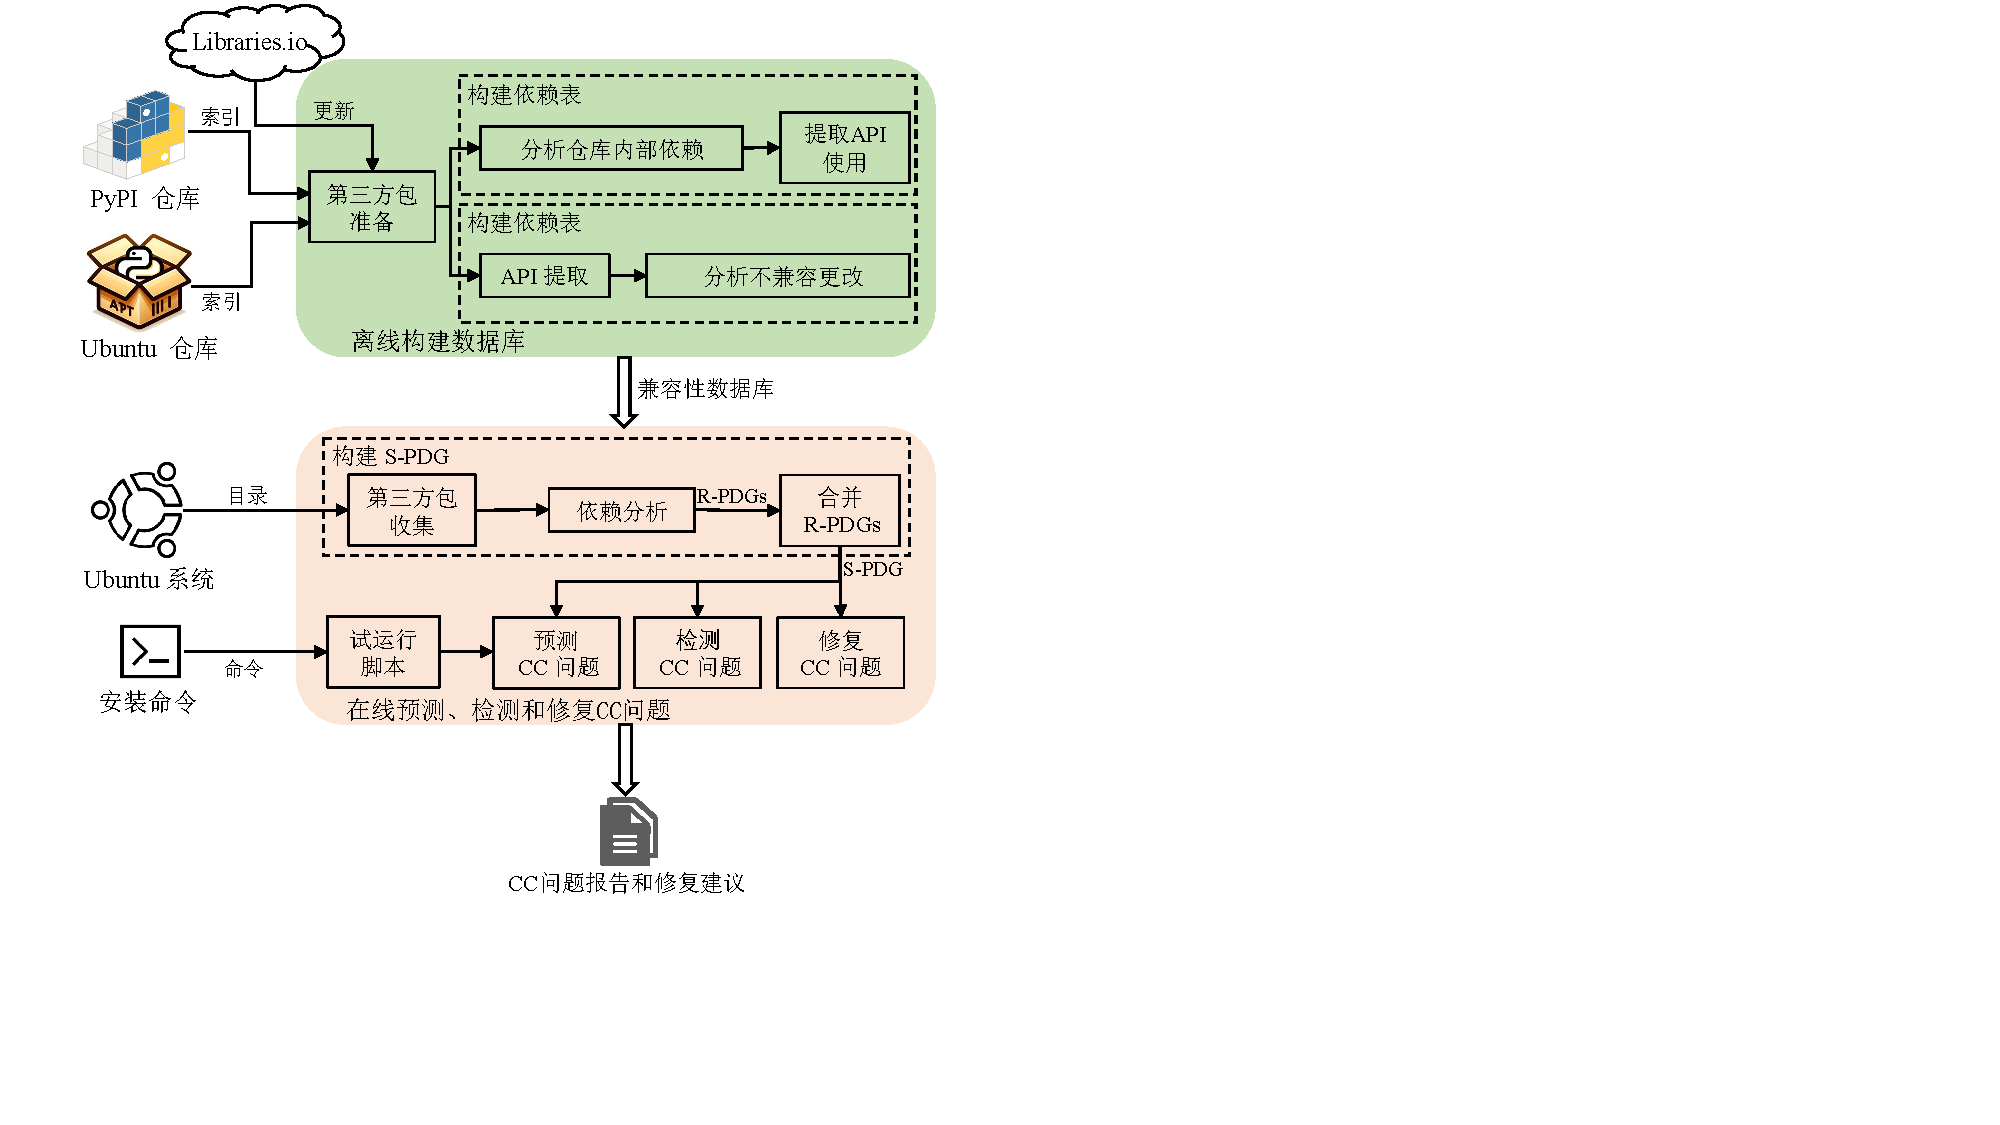
\includegraphics[width=5in]{overview2}
	\caption{\tool{}的总体框架图}
	\label{fig:overview}
\end{figure}
\tool{}主要包括离线和在线两个阶段,离线阶段负责构建一个兼容性数据库,在线阶段负责预测、检测和修复CC问题,包括两个主要表格:依赖表和兼容性表(见第 \ref{4.1}节)。在线阶段构建了一个系统级软件包依赖图(S-PDG),用于检测和预测 CC 问题,并提供修复建议(见第 \ref{4.2} 节)。

\section{构建兼容性数据库}\label{4.1}
由于 \tool{} 旨在用户的生产环境中工作,因此其性能开销至关重要。然而,在线分析所有应用软件包和库软件包之间的兼容性需要较高的开销。为了克服这一限制,我们基于第 \ref{3.3} 节中 CC 问题的特性,将应用软件包与库软件包之间的兼容性问题转化为同一库软件包在 apt 仓库和 pip 仓库中的兼容性问题。例如,在图 \ref{fig:command} 中,应用软件包 “amp” 与库软件包 “numpy” 之间存在 CC 问题。由于 “amp” 与库软件包 “numpy 1.17.4” 兼容,我们可以通过分析 “numpy 1.17.4” 与 “numpy 1.24.3” 的 API 兼容性以及 “amp” 是否调用了破坏性 API 来确定 “amp” 与 “numpy 1.24.3” 的兼容性。

为了实现这一目标,我们在离线阶段构建了一个跨仓库兼容性数据库,从而避免在线阶段进行复杂的程序分析。该兼容性数据库包含依赖表和兼容性表。对于 apt 仓库中的每个应用软件包,依赖表收集其在 apt 仓库中每个库软件包的 API 使用情况。对于 apt 仓库中的每个库软件包,兼容性表收集了其与 pip 仓库中同一软件包各个版本的 API 兼容性。构建过程首先从两个仓库索引的软件包中准备应用软件包和库软件包(见第 \ref{4.1.1} 节),然后通过 API 使用提取构建依赖表(见第 \ref{4.1.2} 节),最后通过兼容性分析构建兼容性表(见第 \ref{4.1.3} 节)。

\subsection{第三方包准备}\label{4.1.1}
我们的研究首先关注了从 apt 仓库中收集应用软件包的过程。以 Ubuntu 20.04 为例,该发行版共维护了 3,319 个 Python 软件包。我们利用 apt 工具获取了这些软件包的源代码,旨在进行 API 使用情况的提取与分析。随后,我们探讨了这些应用软件包是否在 Python 的中央仓库 PyPI \upcite{pypi} 中也有对应的条目。PyPI 仓库本身包含了超过 40 万个第三方 Python 软件包,它是 Python 社区中最大的第三方包中央仓库。

具体而言,我们从 PyPI 中检索了每个软件包的可安装版本。如果存在可安装版本,我们将其视为库软件包,并使用 pip 下载该软件包的所有版本源代码。然而,由于两个中央仓库中的命名策略不同,同一个 Python 软件包可能在这两个仓库中有不同的名称。为了解决这个问题,我们获取了每个应用软件包的顶级模块名称,并使用该名称在 PyPI 中匹配软件包,从而避免遗漏。通过这种方式,我们共识别了 2,419 个库软件包及其在 PyPI 中的所有可安装版本。

每个库软件包拥有两份版本信息,一份是apt能安装的固定版本,另一份是pip能安装的版本集合,将二者进行映射可以更方便的进行后续分析,但是由于两个软件源的包版本编号逻辑不一致,无法直接根据版本号进行这个过程。表\ref{tab:version}中列举了两个库软件包版本映射的例子,numpy的apt安装的版本为“1:1.17.4-5ubuntu3”,在PyPI中对应为“1.17.4”,bip32utils的apt安装的版本为“0.0~git20170118.dd9c541-2”,在PyPI中对应为“0.3.post3”。为了解决这个问题,我们利用Python包检查工具pip-check\upcite{pip-check},来帮助我们准确的进行版本映射。
\begin{table}
	\centering
	\begin{threeparttable}
		\caption{库软件包版本映射的例子}
		\label{tab:version}
		\begin{tabularx}{0.66\textwidth}{ccc}
			\toprule
			\textbf{库软件包}&\textbf{apt安装的版本}&\textbf{PyPI中对应的版本}\\
			\midrule
			numpy&1:1.17.4-5ubuntu3&1.17.4\\
			bip32utils&0.0~git20170118.dd9c541-2&0.3.post3\\
			\bottomrule
		\end{tabularx}
	\end{threeparttable}
\end{table}

由于库软件包在 PyPI 中不断更新和演进,维护一个实时更新的数据库是必要的。然而,手动更新这样的数据库是不现实的,特别是考虑到 PyPI 更新的频繁性。因此,我们采用了 \textit{Libraries.io} \upcite{libraries.io} 平台的服务,该平台监控了包括 PyPI 在内的 32 个生态系统中的库更新。利用这一平台,我们能够自动化地捕捉最新的软件包版本,实现兼容性数据库的增量更新,从而确保数据的时效性和准确性。这不仅提高了我们研究的效率,也增强了研究结果的应用价值。

\subsection{依赖表构建}\label{4.1.2}
依赖表存储了所有应用软件包在 apt 仓库中库软件包的 API 使用情况。依赖表的存储格式如图\ref{fig:dependency}所示。
\begin{figure}[htbp] % use float package if you want it here
	\centering
	
\includegraphics[width=3in]{依赖表}
	\caption{依赖表示例}
	\label{fig:dependency}
\end{figure}
数据分析过程分为以下两个步骤:
\begin{itemize}
	\item \textbf{步骤 1:分析 apt 仓库的内部依赖关系。}apt 仓库中的所有应用软件包都依赖于 apt 仓库中库软件包的预定义版本。因此,分析 apt 的内部依赖关系需要检索每个应用软件包所依赖的库软件包。然而,apt 软件包文档将依赖关系分为 \textit{Depends}、\textit{Recommends} 和 \textit{Suggests} 三类。\textit{Depends} 关系是硬性的,即安装时必须满足;而后两者则为软性依赖,可能不会默认安装。为了精确地识别和验证这些依赖关系,我们在隔离的环境中安装每个应用软件包,确保能够精准捕获所有实际的依赖关系,包括那些仅在特定配置或条件下才会触发的依赖。
	\item \textbf{步骤 2:提取库软件包的所有 API 使用情况。}\tool{} 通过静态分析技术来提取 API 的使用情况。首先,对于每个应用软件包及其所有依赖的库软件包,我们遍历应用软件包的源代码文件,检查是否有库软件包的导入语句。一旦确认导入了某个库,\tool{} 则会将源代码解析成抽象语法树(AST)。随后,通过扫描 AST 节点来检测库软件包的 API 调用情况。任何检测到的 API 调用都会被记录在依赖表中,与对应的应用软件包和库软件包关联起来。如果某个应用软件包与库软件包之间没有直接的 API 调用,但存在间接依赖,这种情况也将被记录,以揭示潜在的隐蔽依赖关系。
\end{itemize}
通过这两个步骤,我们能够构建一个全面的依赖表,为后续的兼容性分析提供强有力的数据支持。

\subsection{兼容性表构建}\label{4.1.3}
兼容性表存储了每个库软件包与 pip 仓库中同一软件包各版本之间的 API 兼容性。兼容性表的存储格式如图 \ref{fig:compatibility} 所示。
\begin{figure}[htbp] % use float package if you want it here
	\centering
	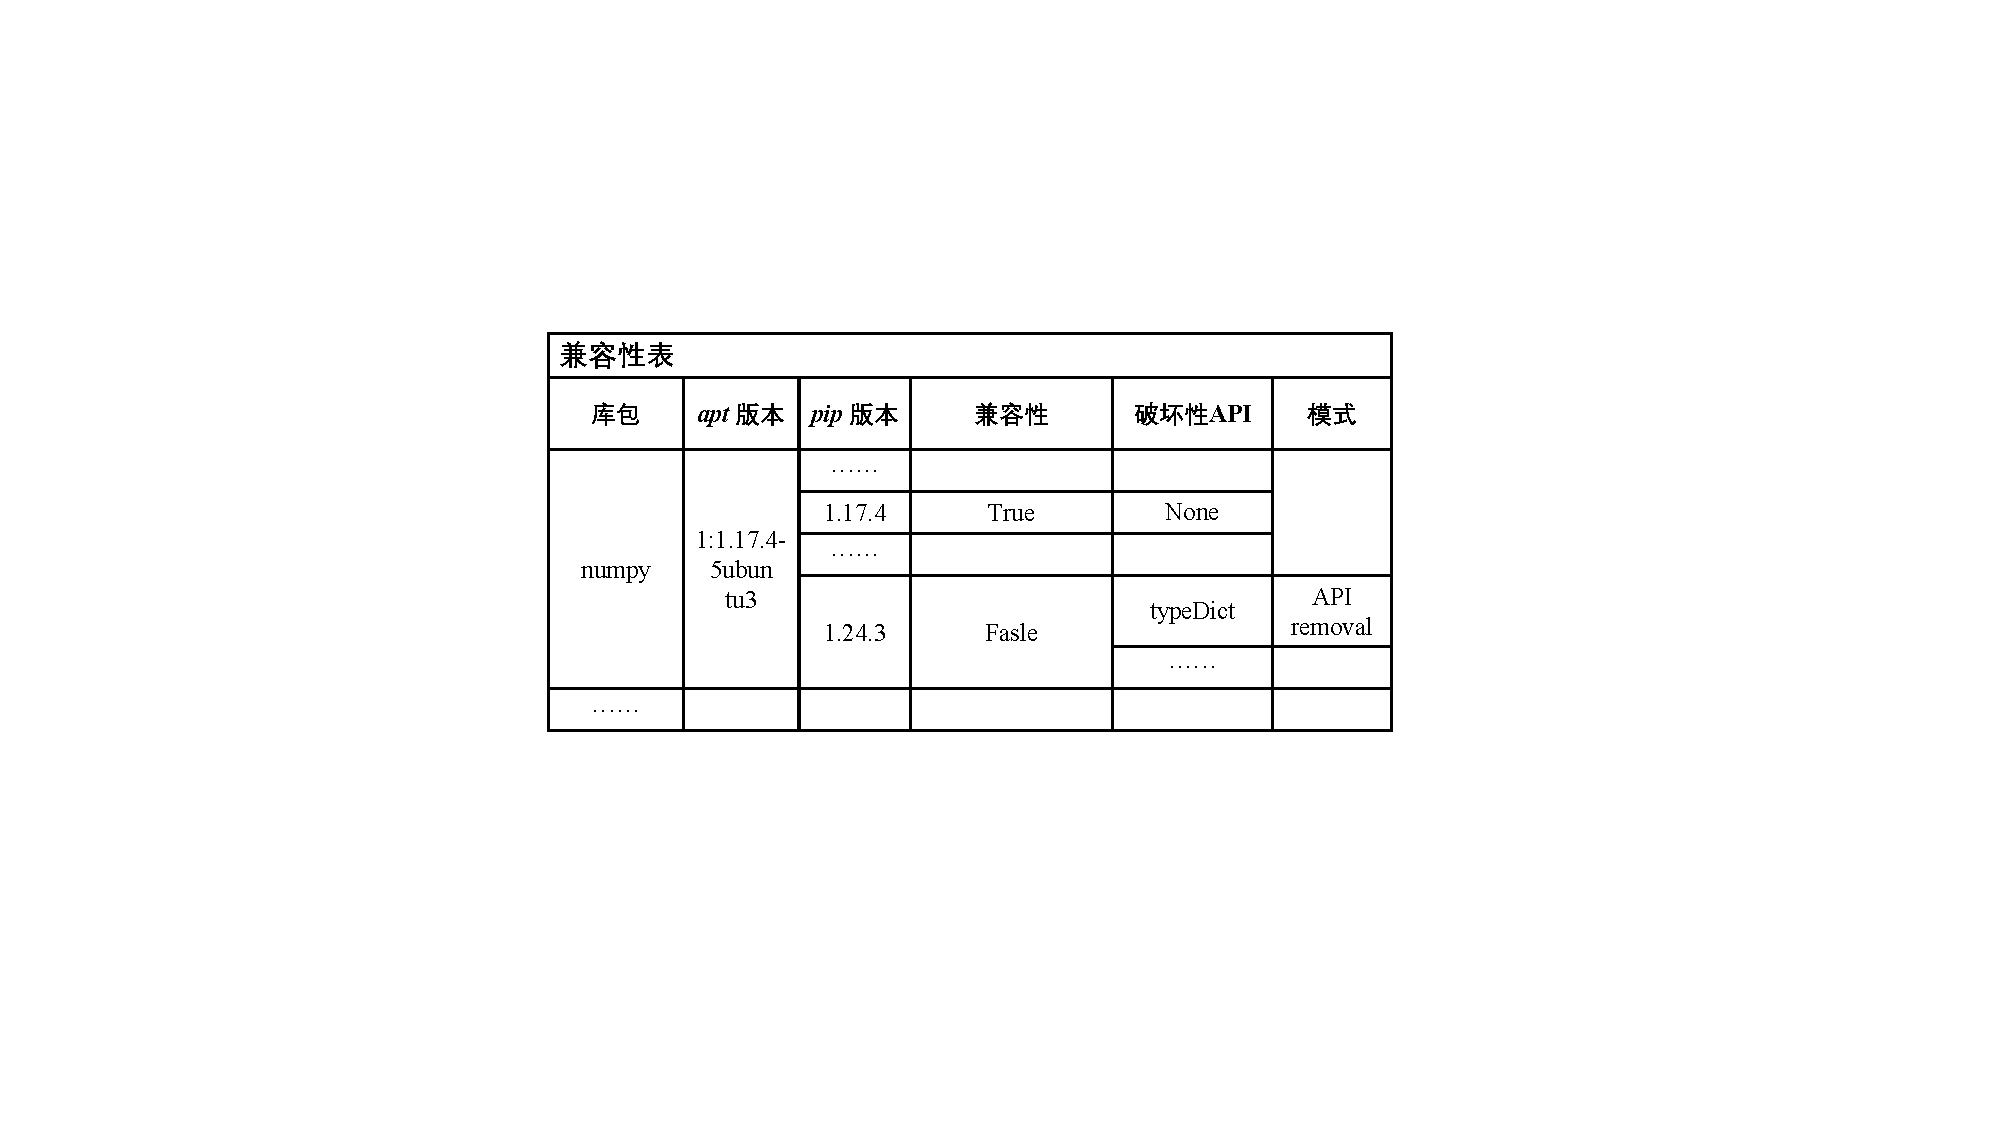
\includegraphics[width=5in]{兼容性表}
	\caption{兼容性表示例}
	\label{fig:compatibility}
\end{figure}如果库软件包的不同版本之间存在 API 不兼容的更改,\tool{} 会在兼容性表中记录它们之间的不兼容关系及所有不兼容的 API。为了实现这一目标,\tool{} 执行了以下两个步骤:
\begin{itemize}
	\item \textbf{步骤 1:API提取。}为了准确分析库软件包不同版本之间的兼容性,首先需要获取该库软件包各版本的所有 API。对于大多数静态编程语言,静态分析可以有效地提取软件包提供的 API。然而,Python 是一种动态编程语言,一些 API 由 Python 对象在运行时创建和修改,无法通过静态分析获取。为了解决这一问题,我们采用了动态分析与静态分析相结合的策略来提取 API,涵盖了类、函数(及其参数)和属性等。在动态分析中,我们使用 \textit{inspect} 模块在导入 Python 软件包后进行反射动态 API 提取。\textit{inspect} 模块能够动态访问活动对象的内部结构,从而提取由 Python 对象在运行时创建和修改的 API。此外,我们使用 \textit{parso} \upcite{parso} 模块进行静态分析,以补充函数定义和其他信息的提取。
	
	\begin{table*}
	\centering
	\begin{threeparttable}
		\caption{判定API不兼容更改的规则}
		\begin{tabularx}{\textwidth}{clXrc}
			\hline
			%\small
			\textbf{序号} &\textbf{更改模式}&\textbf{规则}&\textbf{频率}&\textbf{IC类型}\\ 
			\hline
			1 & API\_addition &$API \notin API_{old} \land API \in API_{new} $&32,674,616 (77.69\%)&$BIC$\\
			2 & API\_removal & $API \in API_{old} \land API \notin API_{new} $ & 8,831,893 (21.00\%) &$FIC$\\
			3 & Param\_addition &$API\in API_{old} \cap API_{new}\land p \notin P_{old} \land p \in P_{new} \land p \notin OP_{new}$ & 102,490 (0.24\%)&$BIC/FIC$ \\
			4 & Param\_removal &$API\in API_{old} \cap API_{new}\land p \in P_{old} \land p \notin OP_{old}\land p \notin P_{new}$ & 71,221 (0.17\%)&$BIC/FIC$ \\
			5 & Optional\_param\_addition &$API\in API_{old} \cap API_{new}\land p \notin OP_{old} \land p \in OP_{new}$ &328,988(0.78\%) &$BIC$  \\
			6 & Optional\_param\_removal &$API\in API_{old} \cap API_{new} \land p \in OP_{old} \land p \notin OP_{new} $ & 46,275(0.11\%) &$FIC$ \\
			7 & Param\_reordering &$API\in API_{old} \cap API_{new} \land rp(p,P_{old}, OP_{old}) \neq rp(p,P_{new}, OP_{new})$& 3,973 (0.01\%) &$BIC/FIC$\\
			\hline
		\end{tabularx}
		\begin{tablenotes}[flushleft]
			\small 
			\item “API” 表示单个 API,而 “$API_{old/new}$” 表示 API 集合。“p” 表示单个参数,“$P_{old/new}$” 表示必选参数列表,"$OP_{old/new}$" 表示可选参数列表。“$rp(p, P_{old/new}, OP_{old/new})$” 表示 “p” 在参数列表中的相对位置。
		\end{tablenotes}
		\label{tab:rules}
	\end{threeparttable}
	% \vspace{-2mm}
\end{table*}
	\item \textbf{步骤 2:分析API不兼容更改。}准确分析库软件包不同版本之间的不兼容更改(IC)是 \tool{}有效性的保证。不兼容更改包括两种类型:前向不兼容更改(FIC)(例如,添加一个 API)和后向不兼容更改(BIC)(例如,移除一个 API)\upcite{jia2021depowl}。由于在 CC 问题中,apt 仓库和 pip 仓库中的库软件包版本顺序不一定是连续的,因此这两种类型的不兼容更改都可能导致软件包不兼容,并引发 CC 问题。作为不兼容更改分析目标的 Python 拥有灵活的语法,因此其 API 更改的复杂性远超 C++ 和 Java 等语言。因此,很难确定哪些 API 更改是属于不兼容的。
	
	为了解决这一问题,我们借鉴了现有研究 \cite{zhang2020python},考虑了 前向不兼容更改 和 后向不兼容更改 两种类型,总结了七种不兼容更改模式,并设计了判定规则。这些模式和规则如表 2 所示,频率表示兼容性表中每种模式的占比。对于与 API 相关的更改,我们根据 API 提取步骤的结果检测 Python 程序中类、函数和属性的添加或删除。对于与 API 参数相关的更改,我们考虑了必选参数和可选参数的变动以及参数顺序的变动。值得注意的是,从必选参数变为可选参数(或反之)将由规则 3(4)检测到。我们将发生不兼容更改的 API 称为破坏性 API。兼容性表将存储每个不兼容更改的破坏性 API 信息,包括名称、参数、类型和更改模式等。

\end{itemize}

基于上述两个步骤,在 Ubuntu 20.04 和 Python 3.8.10 环境中,我们从 2,419 个库软件包的 47,387 个版本中提取了 62,552,811 个 API,并发现了 42,059,456 个API不兼容更改。

\section{预测、检测和修复CC问题}\label{4.2}
CC问题涉及到软件包管理工具和Python解释器之间的复杂交互,这些问题的预测、检测和修复因而具有一定的挑战性。为了有效处理这一挑战,我们提出了一个系统级软件包依赖图(System-level Package Dependency Graph, S-PDG),该图用于描述apt、pip和Python解释器之间的交互关系。在本节中,我们主要解释如何构建 S-PDG(见第 \ref{4.2.1} 节),并将其与跨仓库兼容性数据库结合使用来检测 CC 问题(见第 \ref{4.2.2} 节)。我们还解释了如何通过模拟运行命令来预测 CC 问题(见第 \ref{4.2.3} 节)并为用户提供修复 CC 问题的建议(见第 \ref{4.2.4} 节)。
\subsection{构建S-PDG}\label{4.2.1}
首先,\tool{}会收集 系统本地apt 和 pip仓库中的Python第三方包并分析目录内部包依赖关系,构建两个仓库级软件包依赖图(R-PDG),本节将本地apt 和 pip仓库称为apt 和 pip目录。然后,\tool{}会将这两个 R-PDG 合并为一个 S-PDG,并检测 CC 问题。S-PDG 的构建过程如算法\ref{alg:BuildSPDG}所示,主要分为以下三个步骤:
\begin{algorithm}[htbp]
	\caption{构建系统级软件包依赖图 (S-PDG)}
	\label{alg:BuildSPDG}
	\begin{algorithmic}[1]
		\REQUIRE apt directory, pip directory
		\ENSURE System-level Package Dependency Graph (S-PDG)
		
		\STATE {\bfseries Step1: Collect packages from apt and pip directories:}
		\STATE $apt\_pkg$ = get\_packages\_from\_apt\_dir(apt directory)
		\STATE $pip\_pkg$ = get\_packages\_from\_pip\_dir(pip directory)
		
		\STATE {\bfseries Step2: Build R-PDG:}
		\STATE $apt\_RPDG$ = construct\_RPDG($apt\_pkg$)
		\STATE $pip\_RPDG$ = construct\_RPDG($pip\_pkg$)
		
		\STATE {\bfseries Step3: Merge R-PDGs to construct S-PDG:}
		\STATE Initialize $S\_PDG$ as empty graph
		\FOR{each package $A$ in $apt\_RPDG$}
		\IF{$A$ also exists in $pip\_RPDG$}
		\STATE Add a covered edge in $S\_PDG$ from $A$ in $apt\_RPDG$ to $A$ in $pip\_RPDG$
		\ELSE
		\STATE Add $A$ to $S\_PDG$
		\ENDIF
		\ENDFOR
		\FOR{each package $P$ exclusively in $pip\_RPDG$}
		\STATE Add $P$ to $S\_PDG$
		\ENDFOR
	\end{algorithmic}
\end{algorithm}

\begin{itemize}
	\item \textbf{步骤 1:收集 apt 和 pip 目录中的软件包。}对于 apt 目录,\tool{} 使用 dpkg \upcite{dpkg} 工具(一个适用于基于 Debian 系统的底层包管理工具)根据软件包安装记录收集 apt 目录中的所有软件包。pip 提供了类似的功能,但它只能从所有系统级目录中收集软件包,无法指定只从 pip 目录中收集软件包。为了解决这个问题,\tool{} 使用 \textit{pkg\_resources} 模块根据目录路径从 pip 目录中收集所有软件包。\textit{pkg\_resources} 是一个 Python 库,用于发现和访问在环境中安装的软件包的资源,它提供了一种便捷的方式来查询包信息和管理运行时依赖关系。
	\item \textbf{步骤 2:分析依赖关系并构建 R-PDG。}在该步骤中,\tool{} 分析了 apt 和 pip 目录内部的依赖关系,并构建了两个仓库级软件包依赖图(R-PDG)。R-PDG 是一个有向无环图,其中节点表示软件包,有向边表示目录内软件包之间的内部依赖关系,本文将其视为兼容的依赖关系。对于 apt 目录,由于系统内apt仓库中的所有包均为固定版本和固定依赖关系的,\tool{}利用第 \ref{4.1.2} 节中获得的 apt 仓库内部依赖关系图,将其进行子图分割从而构建 R-PDG。对于 pip 目录,\tool{}利用依赖分析工具 pipdeptree \upcite{pipdeptree} 来分析 pip 目录内部的依赖关系,并构建 R-PDG。Pipdeptree 是一个 Python 工具,用于查看已安装的 pip 软件包的依赖关系树,帮助开发者可视化和理解包之间的依赖关系。
	\item \textbf{步骤 3:合并 R-PDG 以构建 S-PDG。}\tool{}通过合并两个 R-PDG 构建了系统级软件包依赖图(S-PDG)。图 \ref{fig:PDG} 展示了合并两个 R-PDG 以构建一个 S-PDG 的示意图,其中软件包 B 和 D 在 apt 和 pip 目录中各有一个版本。当一个软件包在两个 R-PDG 中各有一个版本时,\tool{} 在S-PDG中会添加一条边连接这两个版本,表示 apt 中的版本被 pip 中的版本覆盖。该边从 apt R-PDG 中的节点指向 pip R-PDG 中的节点,称为覆盖边(covered-edge)。根据\ref{3.2.2}分析的Python 解释器的导入规则,被覆盖的版本将不再被使用,因此依赖于被覆盖包的应用包有可能发生CC问题。
	\begin{figure}[t] % use float package if you want it here
		\centering
		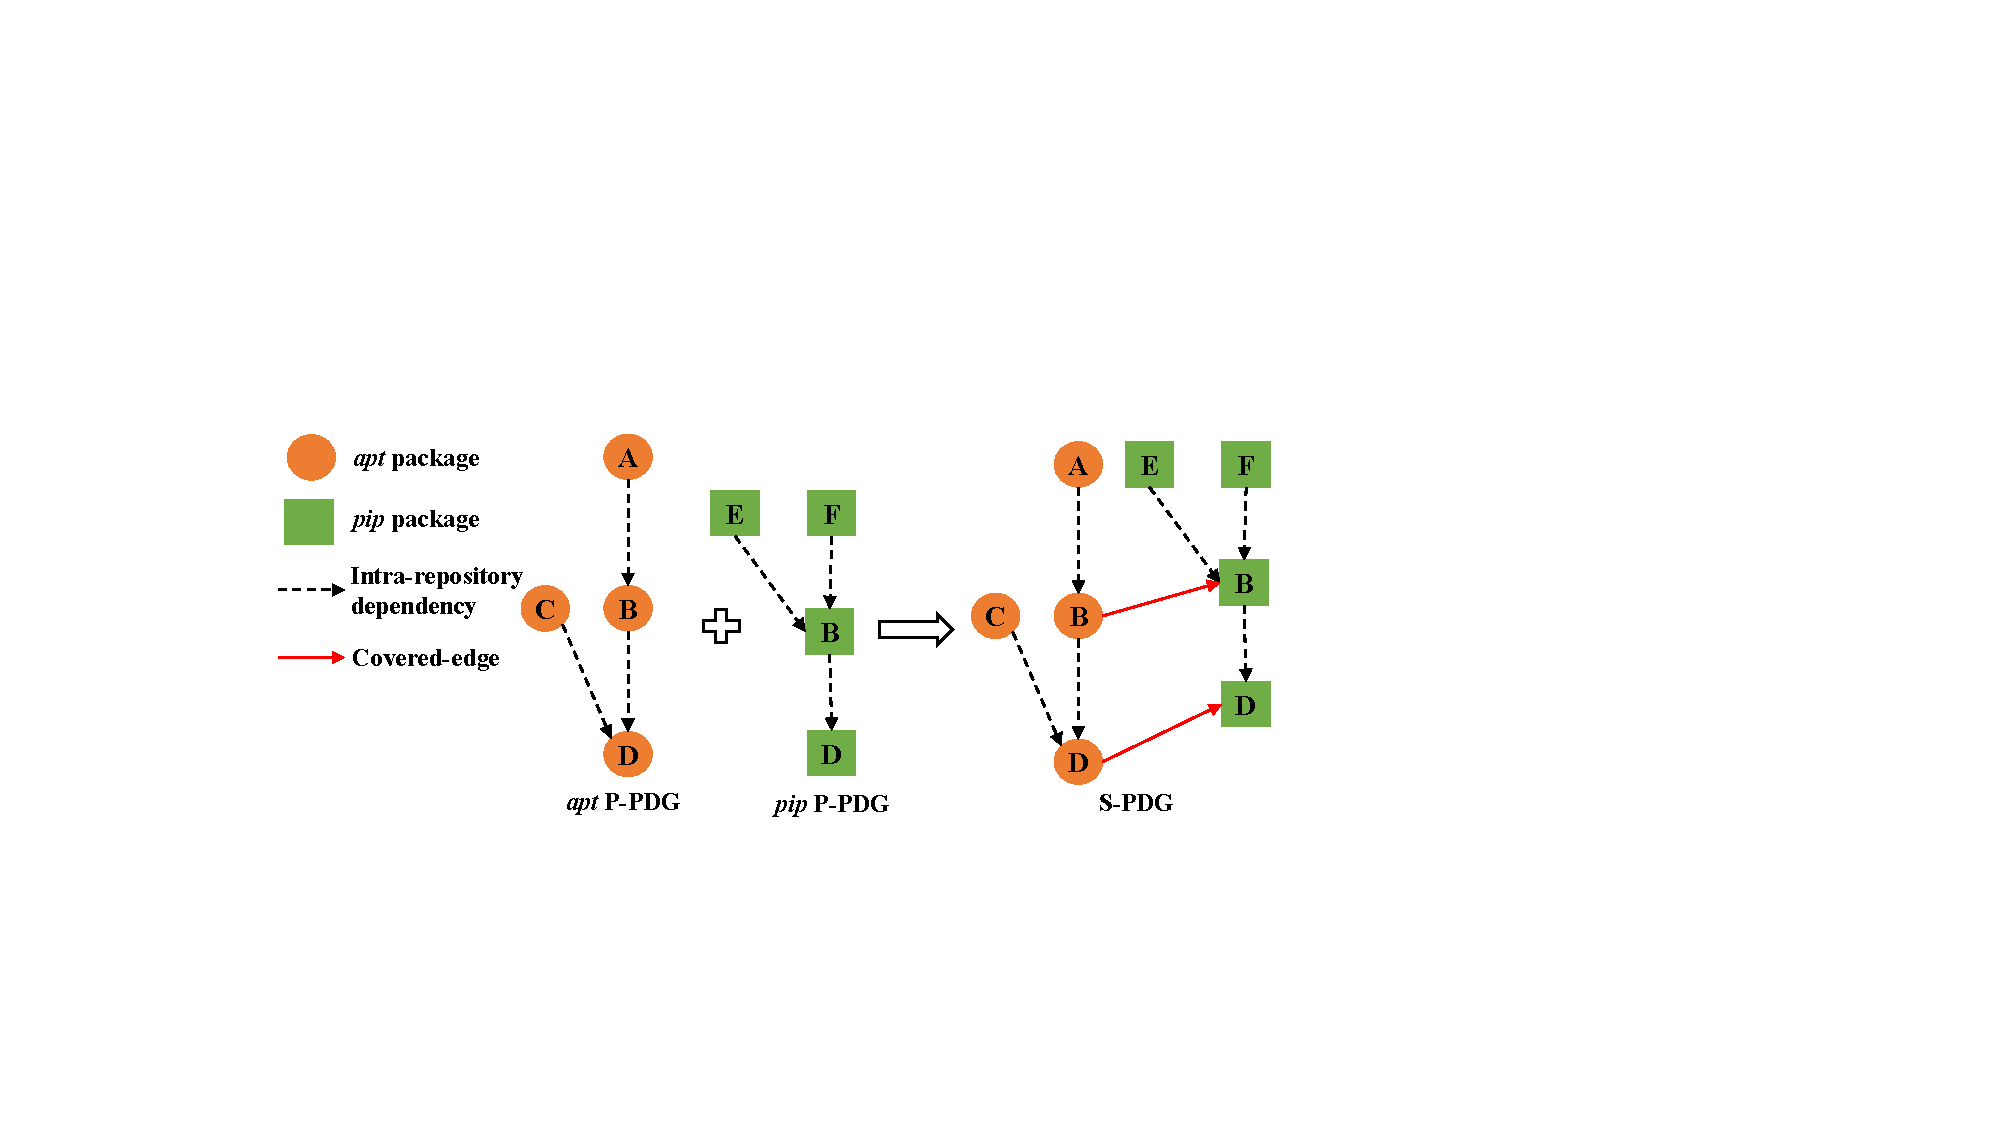
\includegraphics[width=5in]{chain}
		\caption{合并两个 R-PDG 构建S-PDG示意图}
		\label{fig:PDG}
	\end{figure}
	
\end{itemize}
\subsection{检测CC问题}\label{4.2.2}
构建 S-PDG 后,我们可以在用户的系统环境中检测 CC 问题,算法\ref{alg:DetectCC}展示了检测流程。为了实现这一点,\tool{} 会查询兼容性表,以确定每条覆盖边连接的两个版本之间是否存在破坏性 API(例如,图 \ref{fig:PDG} 中软件包 B 和 D 的两个版本之间)。如果存在,说明用户系统中包含不兼容的库软件包版本,可能导致潜在的 CC 问题为了确认潜在问题,\tool{} 会查询依赖表,检查 apt 目录中的应用软件包是否使用了该破坏性 API(例如,检查图 \ref{fig:PDG}中的软件包 A 和 C)。如果存在,\tool{} 将报告一个 CC 问题。
\begin{algorithm}[htbp]
	\caption{检测CC问题}
	\label{alg:DetectCC}
	\begin{algorithmic}[1]
		\REQUIRE System-Level Package Dependency Graph (S-PDG), Compatibility Table, Dependency Table
		\ENSURE List of detected CC issues
		
		\STATE Initialize an empty list of CC issues
		\FOR{each covered edge $(A, B)$ in S-PDG}
		\STATE $A_{version} \gets$ Version of package $A$ in apt
		\STATE $B_{version} \gets$ Version of package $B$ in pip
		\STATE Check the Compatibility Table for $A_{version}$ and $B_{version}$
		\IF{incompatibilities exist}
		\STATE Query the Compatibility Table for APIs incompatible between $A_{version}$ and $B_{version}$
		\STATE $incompatibleAPIs \gets$ List of incompatible APIs
		\FOR{each $api$ in $incompatibleAPIs$}
		\STATE Check the Dependency Table to see if $api$ is used by $package$ $A$
		\IF{$api$ is used by $package$ $A$}
		\STATE Add "CC issue detected with $api$ in package $A$" to list of CC issues
		\ENDIF
		\ENDFOR
		\ENDIF
		\ENDFOR
		\RETURN List of CC issues
	\end{algorithmic}
\end{algorithm}


\subsection{预测CC问题}\label{4.2.3}
在预测阶段,\tool{} 通过模拟运行安装命令,并将要安装的软件包临时添加到 S-PDG 中。具体而言,对于每个 apt 或 pip 的安装命令,\tool{} 使用 “apt install -s” 或 “pip install --dry-run” 命令来预览将要安装的软件包。随后,\tool{} 将这些软件包临时添加到 S-PDG 中,并检查是否需要添加新的覆盖边。如果需要添加新的覆盖边,\tool{} 会查询兼容性表和依赖表,检测是否会引发新的 CC 问题。如果会引发 CC 问题,\tool{} 会警告用户执行该安装命令会导致 CC 问题,并报告预测的 CC 问题的详细信息,如覆盖边两端的相关软件包。该预测机制能够有效防止在安装过程中引入 CC 问题。

\subsection{修复CC问题}\label{4.2.4}
当检测到 CC 问题时,由于 R-PDG 中包含兼容的依赖关系,\tool{} 可以据此提供修复建议。
通常有两种方法可以解决 CC 问题:a) 通过删除并重新安装软件包来断开 S-PDG 中的覆盖边,b) 指定从 apt 目录中导入兼容的库软件包。由于方案 a 可能会导致其他系统级依赖问题,因此我们推荐使用方案 b 来修复 CC 问题。基于 apt 目录的 R-PDG,\tool{} 会建议用户在导入应用软件包之前,使用 \textit{importlib} 模块从 apt 目录导入兼容的库软件包。

\section{本章小结}
本章深入探讨了 \tool{}的设计与实现,这是一个旨在预测、检测和修复CC问题的自动化工具。 \tool{}主要包括离线和在线两个阶段,离线阶段构建一个兼容性数据库,在线阶段构建一个系统级软件包依赖图,用于检测和预测CC问题,并提供修复建议。\tool{} 能够有效地解决由不同包管理工具安装的第三方包之间发生的兼容性问题。此外,\tool{}提供了一套基于规则的方法来分析库软件包不同版本间的破坏性API更改,本方法结合静态分析和动态分析,能够更有效的识别破坏性API。

总之,本章通过设计和实现\tool{}工具,为解决跨软件生态的兼容性问题提供了思路和解决方案。展望未来,\tool{}工具有望以系统服务的形式集成到操作系统中,进一步推动系统依赖治理技术的发展,特别是在不同软件生态间的第三方包依赖方面。在后续的方面,本文将进一步探讨\tool{}的局限性和可推广性并进行全面的评估。